

\section{Origins of Neuroscience}

The origins of neuroscience date back to pre-history; wherein early hunter-gatherer and nomadic peoples (along with transient civilizations) likely practiced trepenation. Evidence for this can be found in the purposeful boring of holes in the human skull by other humans. It was likely that this was an animist ritual meant to release "evil spirits". In Ancient Egypt the common belief was that the heart was the seat of the soul; rather than the brain. Ancient Greece brought about the birth of neuroanatomy (though crude). Hippocrates, through brain dissections, determined that the brain was an organ which regulated the senses. Socrates conjectured, much like the Egyptians, that the heart was where the self lied, yet it was the brain which radiated the \textit{hot blood} accounting for man's rationality. In the Roman Empire the early neuroanatomist Galen began dissections of animal brains. He discovered that the brain was divided into two subsections: the cerebrum and the cerebellum. 

\begin{figure}[H]
  \begin{center}
    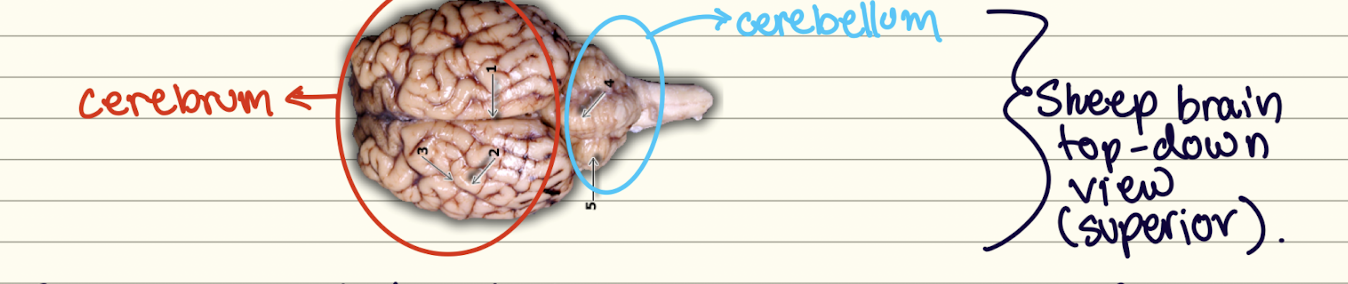
\includegraphics[width=0.95\textwidth]{figures/sheepbrain.png}
  \end{center}
  \caption{}\label{fig:Sheep Brain}
\end{figure}

Galen postulated that the cerebrum must be for memory and sensation since it is soft and impressionable, much like the clay tablets at the time (since soft clay can be impressed with glyphs why should it not be the same for the brain?). Additionally, he concluded that the cerebellum must be for muscle control due to its tough nature. This is a prime example of wrong reasons, right conclusions. Galen further bifurcated brains discovering that there existed hollow, liquid filled cavitied called ventricles: what he surmised to be the four vitual fluids or humors. Sensation and movement, Galen thought, must then have been promlgated by the movement of the humors across and within the ventricles.

\begin{figure}[H]
  \begin{center}
    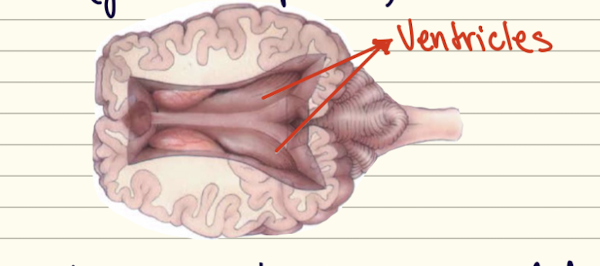
\includegraphics[width=0.50\textwidth]{figures/ventricles.png}
  \end{center}
  \caption{}\label{fig:Ventricles}
\end{figure}

Moving forward in time to The Renaissance, Andreas Vesalius was the first (known) to have created detailed drawings of neuroanatomy based on brain dissections. The humor theory of the brain still remained popular. In 17\ts{th} century France, Ren\'{e} Descartes advocated for the hydraulic-fluid-mechanical theory of brain function. He furthermore posited that mind-body duality (the concept at the time, still beleived by some today, that the mind/self is separate from the body/brain) governed the intellegence of man. In the 19\ts{th} century is when things really start to pop off: it was found that the brain consists of white and gray matter. The former contains fibers which trasmit data to the latter. The gross anatomy of the brain is completed at this time. Additionally, it is found that the bumps and grooves of the brain, now called gyri and sulci, respctively, are identifiable in all normally functioning humans. This led to the parceling of the cerebrum into lobes.  The lobes were called the frontal lobe, temporal lobe, parietal lobe, and occipital lobe.

\begin{figure}[H]
  \begin{center}
    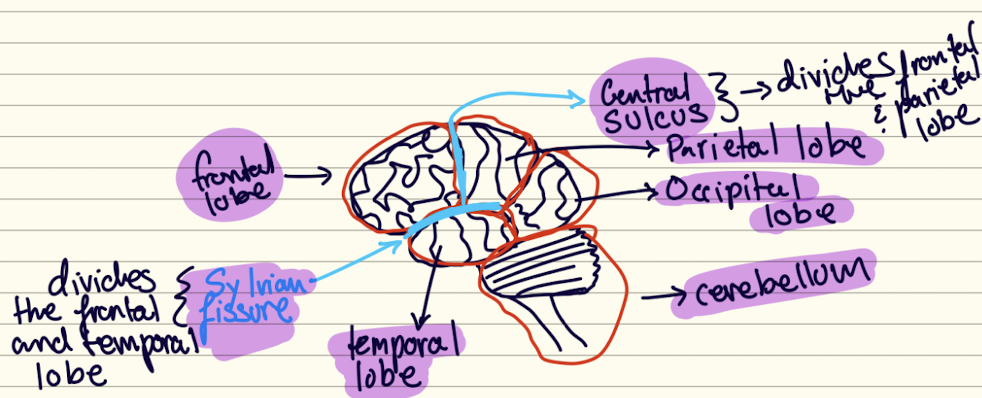
\includegraphics[width=0.95\textwidth]{figures/lobes.png}
  \end{center}
  \caption{}\label{fig:}
\end{figure}

The nervous system was nominatively divided into the central nervous system (CNS), which consisted of the brain and spinal cord, and the peripheral nervous system (PNS), which consisted of the rest of the nervous system.

\begin{figure}[H]
  \begin{center}
    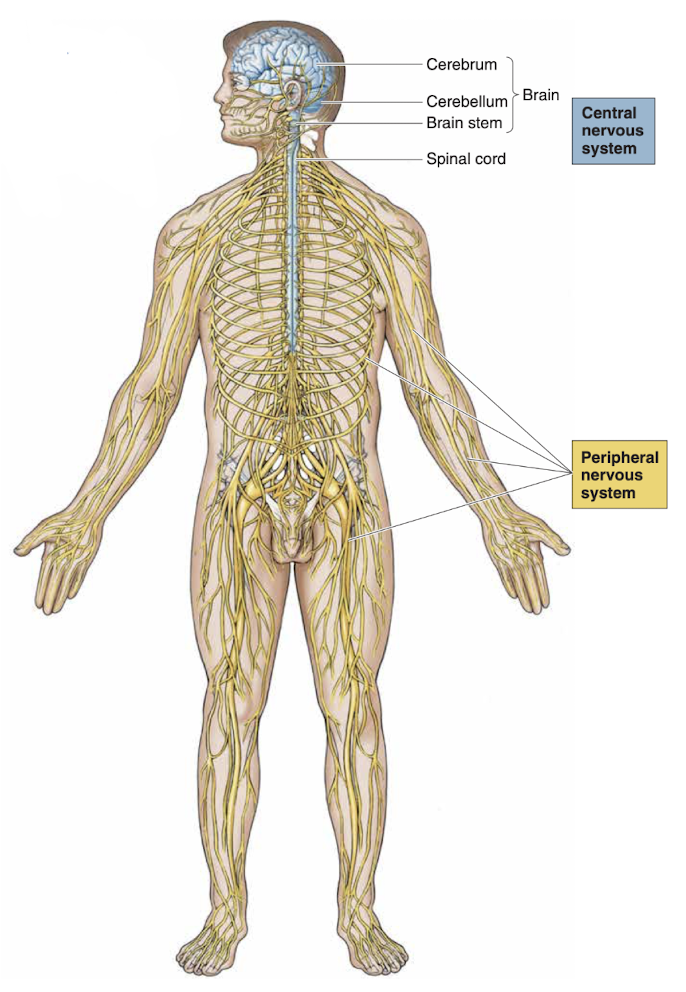
\includegraphics[width=0.35\textwidth]{figures/nerves}
  \end{center}
  \caption{}\label{fig:}
\end{figure}

\pagebreak

To recap all that was understood about the brain up to the end of the 19th century:
\begin{enumerate}
  \item Injury to the brain disrups senses, motor function, and thought;
    
  \item injury to the brain is usually fatal;
  
  \item brain communicates to the body via the nervous system;
  
  \item the brain is made up of smaller sections which have different functions.
\end{enumerate}



